% TU Delft beamer template
% Author: Erwin Walraven (initial version was created by Maarten Abbink)
% Delft Universiy of Technology

\documentclass{beamer}
\usepackage[english]{babel}
\usepackage{calc}
\usepackage[absolute,overlay]{textpos}
\usepackage{graphicx}
\usepackage{subfig}
\usepackage{amsmath}
\usepackage{amsfonts}
\usepackage{amsthm}
\usepackage{mathtools}
\usepackage{comment}
\usepackage{MnSymbol,wasysym}
\usepackage{url}
\usepackage{fancyhdr}
\usepackage{subfig}
\usepackage{xcolor}
\usepackage{subfig}
\usepackage{hyperref}


%colors
\definecolor{mygray}{gray}{0.6}

\setbeamertemplate{navigation symbols}{} % remove navigation symbols
\mode<presentation>{\usetheme{tud}}

% BIB SETTINGS
\usepackage[backend=bibtex,firstinits=true,maxnames=30,maxcitenames=20,url=false,style=authoryear]{biblatex}
\bibliography{bibfile}
\setlength\bibitemsep{0.3cm} % space between entries in the reference list

% Commands
\renewcommand{\bibfont}{\normalfont\scriptsize}
\setbeamerfont{footnote}{size=\tiny}
\renewcommand{\cite}[1]{\footnote<.->[frame]{\fullcite{#1}}}
\newcommand{\sidenote}[1]{{\textcolor{mygray}{\emph{#1}}}}
\renewcommand{\exp}[1]{\langle #1 \rangle} %expectation

\title[]{QAOA: Performance, Mechanics, and Implementation on Near-Term Devices\\Zhou et al. (2018) \\~\\ Paper review }
\subtitle{A Paper by Zhou, Wang, Choi, Pichler and Lukin}
\institute[]{Delft University of Technology, Netherlands}
\author{Joost Bus \\ \tiny{j.c.p.bus@student.tudelft.nl}}
\date{\today}

\begin{document}
{
\setbeamertemplate{footline}{\usebeamertemplate*{minimal footline}}
\frame{\titlepage}
}
{\setbeamertemplate{footline}{\usebeamertemplate*{minimal footline}}}

% Overview
\begin{frame}{Overview}
\tableofcontents
\end{frame}

\section{Questions addressed in this paper}
\begin{frame}{Current problems with QAOA}
	\begin{itemize}
		\item Finding optimal parameters for QAOA is hard / not efficient in $p$
		\item Performance of QAOA beyond its lowest-depth variant ($p=1$) is largely unknown.
	\end{itemize}
\end{frame}

\begin{frame}{What's done in this paper?}
	\begin{enumerate}
		\item Propose heuristic strategies to effieciently optimise the variational parameters $\vec{\gamma}, \vec{\beta}$ by using found patterns from extensive benchmarking. These give quasi-optimal parameters, in the sense that they usually give the global optima. These parameters are found in $O(\text{poly}(p))$ time, as opposed to $2^{O(p)}$ when using (standard) random initalisation.
		\item Benchmark the performance of QAOA and compare it with quantum annealing (Quantum vs. Quantum). Note, the main choke-point in QA is the presence of small spectral gaps.
		\item Resource analysis on the experimental implementation of QAOA with near-term quantum devices.
		%\item A lot more, but that's not directly relevant
	\end{enumerate}
\end{frame}

\section{Quantum and Classical}
\begin{frame}{What part is quantum and what part is classical?}
	\begin{figure}
		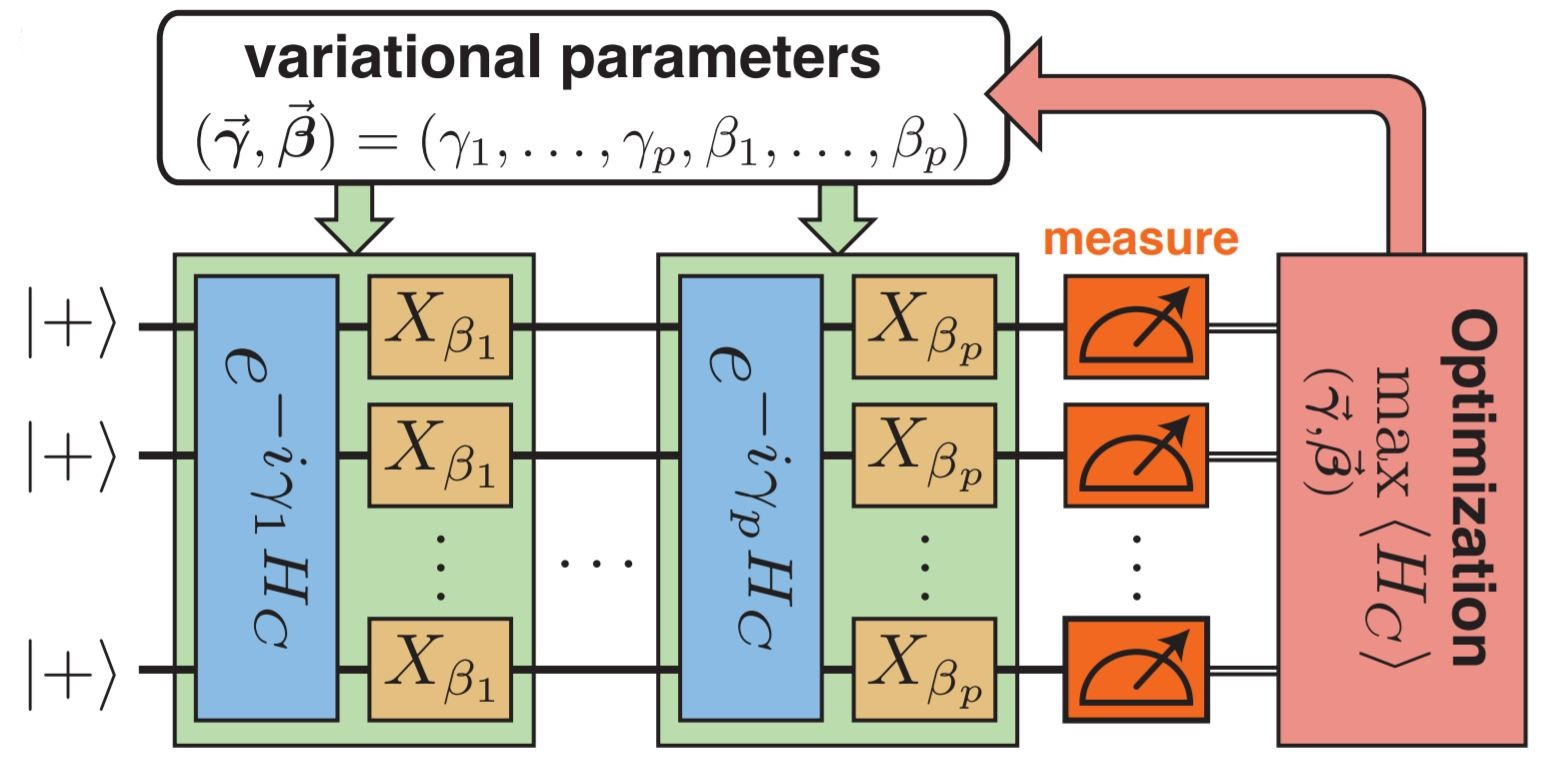
\includegraphics[scale=0.3]{figures/qaoa_idea.JPG}
		\caption{Zhou et al. (2019) page 2}
	\end{figure}	
\end{frame}

\begin{frame}{What part is quantum and what part is classical?}
	We want to maximise the expectation value of the cost function $F_p \equiv \langle \vec{\gamma}, \vec{\beta}| H_C | \vec{\gamma}, \vec{\beta}\rangle$, where $H_C$ is the cost function operator. To estimate this quantity, we make a call to the QPU and take the average over multiple shots.
	We use an optimisation scheme to determine the next parameters that are to be tried. \\~\\ 
	Several optimisation methods are mentioned by Zhou et al. these are
	\begin{itemize}
		\item BFGS
		\item Nelder-Mead \href{https://www.youtube.com/watch?v=HUqLxHfxWqU}{(Visualisation)}
		\item Bayesian Optimisation
	\end{itemize}	

SciPy has an optimisation package that comes in handy, you only need to input the objective function that needs to be optimised, together with an initial point (optionally with other parameters)
\end{frame}

\section{Patterns in the optimal parameters}
\begin{frame}{Patterns in the optimal parameters}
	Randomly initialised optimisation is not efficient in $p$. Zhou et al. instead looked for patterns in the optimal parameters found for u3R, w3R and complete graphs. For u3R graphs they found the following
	\begin{figure}
		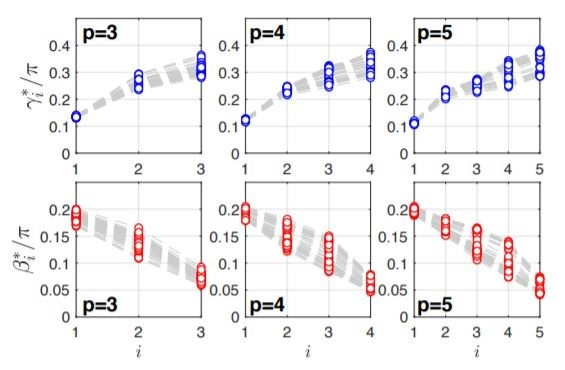
\includegraphics[scale=0.45]{figures/patterns-u3R.jpg}
		\caption{Optimal parameters for randomly generated u3R graphs\\ Zhou et al. (2019) page 4}
	\end{figure}
\end{frame}

\begin{frame}
	Similar patterns were found for w3R and complete graphs.
	\begin{figure}%
		\centering
		\subfloat[w3R graphs]{{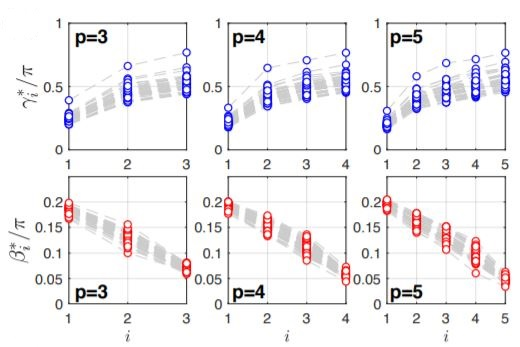
\includegraphics[width=4.5cm]{figures/patterns-w3R.JPG} }}%
		\qquad 
		\subfloat[Complete graphs]{{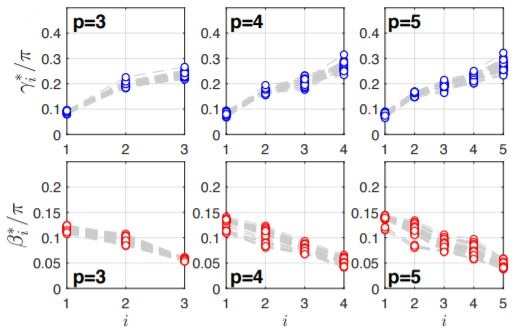
\includegraphics[width=4.5cm]{figures/patterns-complete.JPG} }}%
		\caption{Zhou et al. (2019) page 16 (Appendix)}
	\end{figure}
As can be seen, $\gamma_i$ monotonically increases and $\beta_i$ monotonically decreases. We can exploit this pattern in the optimisation!
\\~\\
Note, this pattern is also reminiscent of the Quantum Adiabatic algorithm, where the mixer hamiltonian $H_B$ is gradually turned off (as $\beta \to 0$), and the cost hamiltonian $H_C$ is gradually turned on.
\end{frame}

\section{Exploiting the patterns}
\begin{frame}{Exploiting the patterns - proposed heuristic methods}
	Zhou et al. proposed two ways to exploit these patterns, these are poetically named
	\begin{enumerate}
		\item INTERP
		\item FOURIER
	\end{enumerate}
	\mbox{ }\\~\\
	Because
	$(\vec{\gamma}^*_{(p+1)}, \vec{\beta}^*_{(p+1)})$ closely resembles $(\vec{\gamma}^*_{(p)}, \vec{\beta}^*_{(p)})$, the idea is to find optimal parameters for low $p$, and from that choose a suitable initialisation for the optimisation for $p+1$ 
\end{frame}

\subsection{INTERP}
\begin{frame}{INTERP}
	INTERP uses linear interpolation to produce a good initial point $(\vec{\gamma},\vec{\beta})$ for optimising the the QAOA parameters as one iteratively increases the level $p$
	
	\begin{equation}
		\Big[\vec{\gamma}_{(p+1)}^0\Big]_i = \frac{i-1}{p}\Big[\vec{\gamma}_{(p)}^L\Big]_{i-1} + \frac{p-i+1}{p}\Big[\vec{\gamma}_{(p)}^L\Big]_i
	\end{equation}
	\begin{equation}
	\Big[\vec{\beta}_{(p+1)}^0\big]_i = \frac{i-1}{p}\Big[\vec{\beta}_{(p)}^L\Big]_{i-1} + \frac{p-i+1}{p}\Big[\vec{\beta}_{(p)}^L\Big]_i
	\end{equation}
	
	for $i = 1, 2, \dots, p+1$. 
\end{frame}
%Where $i$ denotes the $i$th element of the vector and the superscript $0$ denotes the initial point for the next optimisation.

\begin{frame}{INTERP}
	Let's show an example. Suppose we have an (local optimal) set $\vec{\gamma}^L_{(3)} = (\gamma_1, \gamma_2,\gamma_3)$, then we can find a good initial point $\vec{\gamma}^0_{(4)} = (\gamma_1^0, \gamma_2^0,\gamma_3^0, \gamma_4^0)$ using the INTERP method. 
	\begin{figure}%
		\centering
		{{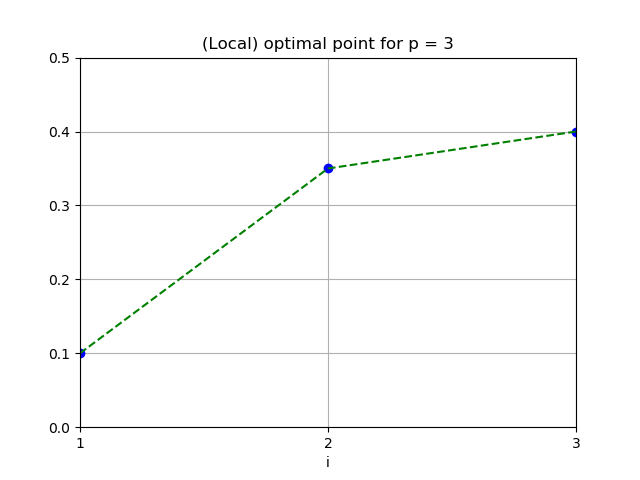
\includegraphics[width=4.75cm]{figures/heuristic_optimal_params.png} }}%
		\qquad 
		{{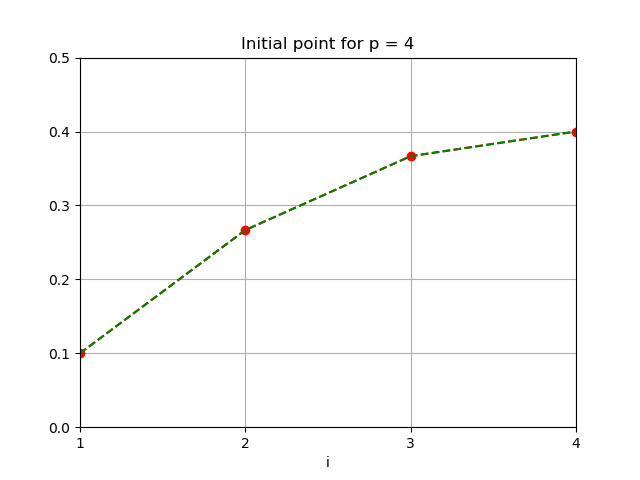
\includegraphics[width=4.75cm]{figures/heuristic_initial_params.png} }}%
		\caption{Illustration of INTERP method}
	\end{figure}
	We can use the same technique for $\vec{\beta}$
\end{frame}

\subsection{FOURIER}
\begin{frame}{FOURIER}
	FOURIER is a somewhat more elaborate technique, but according to Zhou et al. it has a slight edge over INTERP. It's called FOURIER because it makes use of the discrete Fourier and sine transforms. In FOURIER we use a new representation of the $p$-level QAOA parameters using $(\vec{u},\vec{v})\in \mathbb{R}^{2q}$
	\begin{equation}
		\gamma_i = \sum_{k=1}^q u_k \sin \bigg(\Big(k-\frac{1}{2}\Big)\Big(i-\frac{1}{2}\Big)\frac{\pi}{p}\bigg)
	\end{equation}
	\begin{equation}
	\beta_i = \sum_{k=1}^q v_k \cos \bigg(\Big(k-\frac{1}{2}\Big)\Big(i-\frac{1}{2}\Big)\frac{\pi}{p}\bigg)
	\end{equation}
	Here $q$ labels the number of frequency components (and the maximum frequency component) we allow. %Note that when $q=p$ the full power of $p$-level QAOA can be utilised.
\end{frame}

\begin{frame}{FOURIER}
	The strategy works by starting from $p=1$ and then reusing the optimum at level $p$ in $(\vec{u},\vec{v})$-representation to generate a good initial point for level $p+1$
	
	\begin{figure}
		\centering
		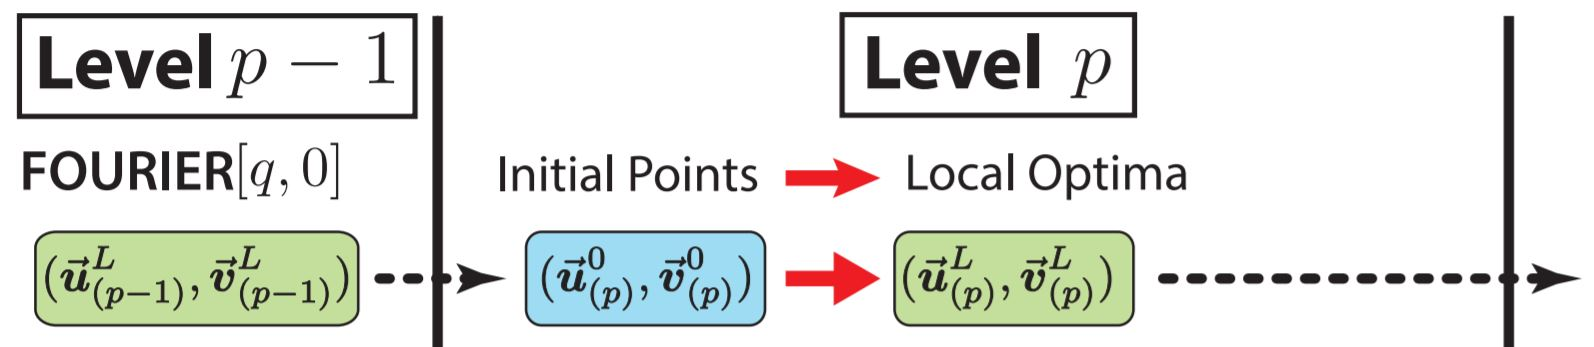
\includegraphics[scale=0.3]{figures/fourier[q,0].JPG}
		\caption{Zhou et al. (2019) page 17 (Appendix)}
	\end{figure}	
	
	Natural choices for $q$ are $p$, but a constant is also possible since the pattern in the optimal parameters seems smooth.
\end{frame}

\begin{frame}{FOURIER[$q=p$,0] a.k.a. FOURIER[$\infty$,0]}
	When $q=p$ we generate new initial points according to
	\begin{equation}
		\vec{u}_{(p+1)}^0 = (\vec{u}_{(p)}^L,0), \quad \vec{v}_{(p+1)}^0 = (\vec{v}_{(p)}^L,0)
	\end{equation}
	All this means is that we generate a good initial point for level $p+1$ by adding a higher frequency component, initialized at zero amplitude.
\end{frame}

\begin{frame}{FOURIER[$q,R$]}
	They proposed several variants of the FOURIER strategy: FOURIER[$q,R$]. This approach uses an extra $R$ random bumps to get out of local optima.
	
	\begin{figure}
		\centering
		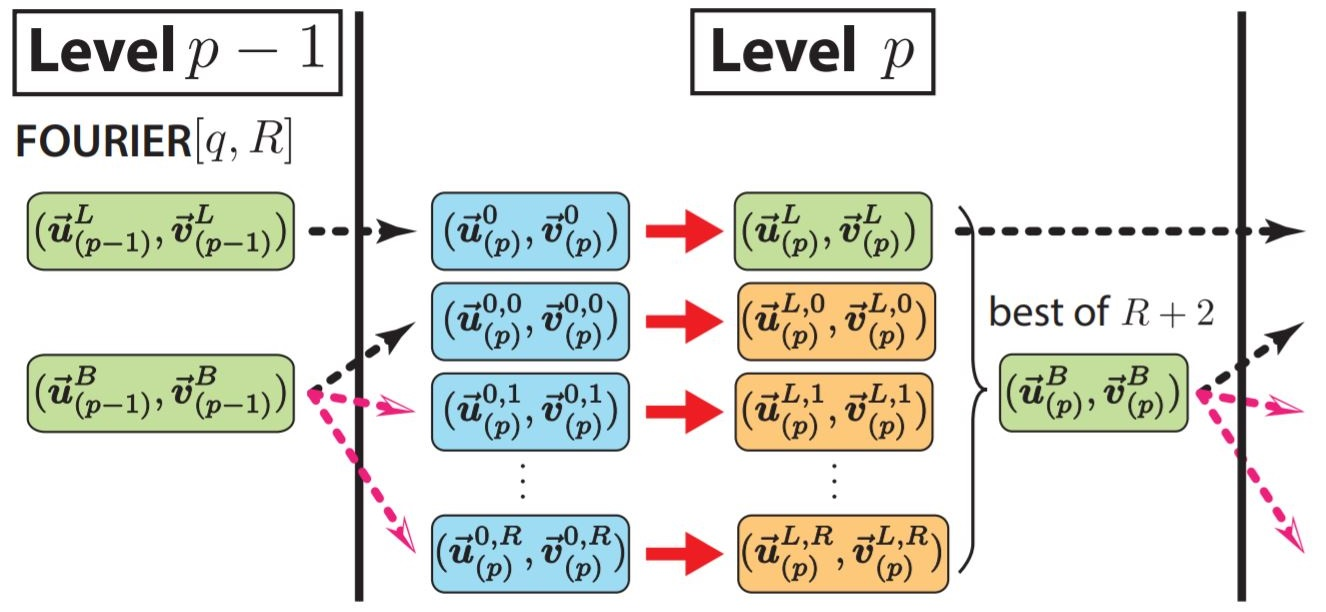
\includegraphics[scale=0.3]{figures/fourier[q,R].JPG}
		\caption{Zhou et al. (2019) page 17 (Appendix)}
	\end{figure}
\end{frame}

\begin{frame}{FOURIER[$\infty,R$]}
	In this variant we perturb the initial point to prevent getting stuck in a local minimum. We do this $R$ times and keep the best set $B$ for the next level $p+1$. For improved robustness of the method we also keep the unperturbed optimized parameters (basically the FOURIER[$\infty,0$] method)
	
	\begin{equation}
			\vec{u}_{(p+1)}^{0,r} = \begin{cases} 
		(\vec{u}^B_{(p)},0) & r = 0 \\
		(\vec{u}^B_{(p)} + \alpha \vec{u}^{P,r}_{(p)}, 0) & 1 \leq r \leq R
		\end{cases}
	\end{equation}
	\begin{equation}
		\vec{v}_{(p+1)}^{0,r} = \begin{cases} 
		(\vec{v}^B_{(p)},0) & r = 0 \\
		(\vec{v}^B_{(p)} + \alpha \vec{v}^{P,r}_{(p)}, 0) & 1 \leq r \leq R
		\end{cases}
	\end{equation}
	where $\vec{u}^{P,r}_{(p)}$ and $\vec{v}^{P,r}_{(p)}$ are the perturbations; randomly drawn numbers from a normal distribution with mean $0$ and variance $|\vec{u}^{B}_{(p)}|^2$, $|\vec{v}^{B}_{(p)}|^2$  respectively. The strength of the perturbation is $\alpha$, according to the paper $\alpha = 0.6$ works well (by trial and error).
\end{frame}

\begin{frame}{Performance of the heuristics}
	\begin{figure}
		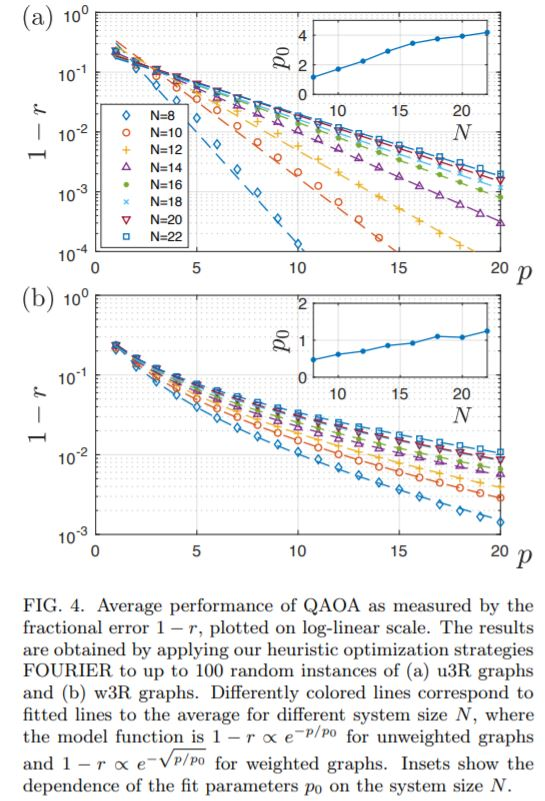
\includegraphics[scale=0.4]{figures/results.JPG}
		\caption{Zhou et al. (2019)}
	\end{figure}
\end{frame}

\begin{frame}{Performance of the heuristics}
\begin{figure}
	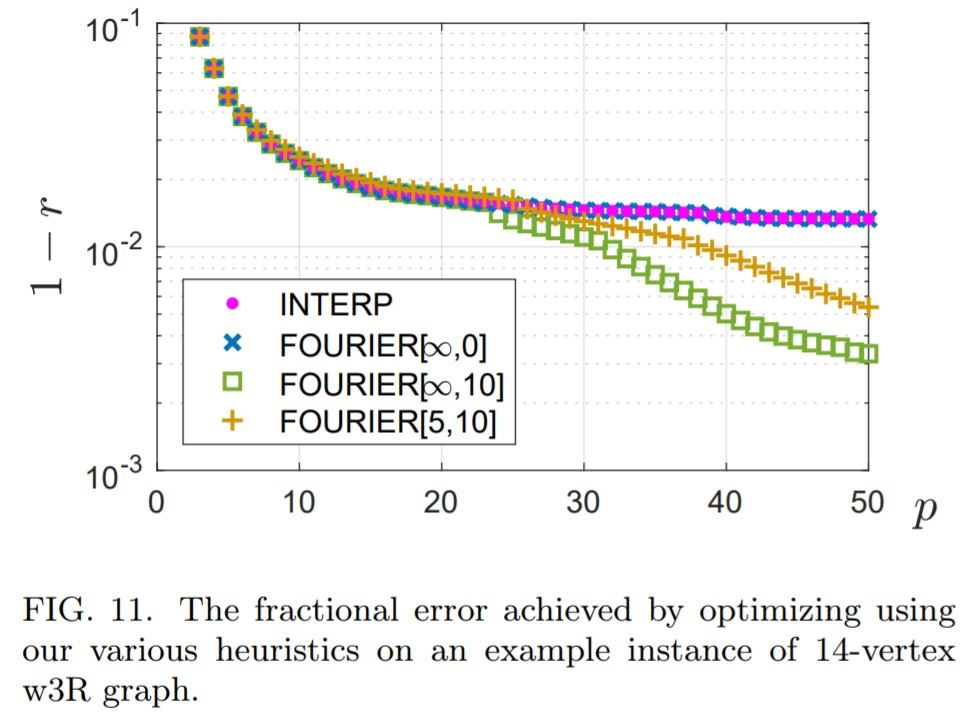
\includegraphics[scale=0.5]{figures/comparison.JPG}
	\caption{Zhou et al. (2019)}
\end{figure}
\end{frame}


\end{document}
